
\chapter{Physics motivation for neutron skin thickness measurement.} \label{intro}
\commento{
\begin{itemize}
\item explain neutron skin thickness.
\item connection to neutron stars radious, and neutron stars description.
\item Equation of state (EoS) for high density nuclear matter.
\item Parity-violating scattering experiment for extracting neutron skin thickness.
\item mention the weak form factor.
\item Transverse asymmetry as background for Parity-violating experiment. 
\item Mention the other experiment, like PREX, that measure zero $A_{n}$ for Lead.
\end{itemize}}

\section{Nuclear equation of state (EOS) and neutron skin thickness.}

\commento{In this section we have to explain what is the neutron skin thickness and why this parameter is related to the Equation of State for nuclear matter (in particular, the slope of the Symmetry energy in the semiempirical mass formula). Then, explain the parallelism between Neutron stars and Nuclear matter (the share the same EOS), and underline the relation between radius of the neutron stars and EOS.}

During the 30s of the last century, a considerable part of the scientific community was concentrated in the study of the structure of atomic nuclei. The discovery that every atoms has a positive charged nucleus dates back to 1908, with the famous Rutherford experiment, where alpha particles scatter from a thin gold foil. In the following years, especially with the birth of quantum mechanics in the second half of the 1920s, significant progress were made in the knowledge of atomic nuclei and their properties. In 1935, a significant contribution was given by Carl Friedrich von Weizsäcker, that proposed the semi-empirical mass formula, to approximate the mass of an atomic nucleus. Although some refinements have been made over the years, the general structure of the formula is the same today. 
The model proposed by Weizsäcker is the application of the liquid-drop model for nuclear matter, where the Nucleus is described as drop of protons and neutrons, that are assumed to be incompressible and are held together by a nuclear potential. The semi-empirical mass formula states that the mass of a nucleus is given by 

\begin{equation}
m = Zm_{p} + Nm_{n} - \frac{E_{B}(N,Z)}{c^{2}}
\end{equation}

An important terms is the binding energy $E_{B}$, that contains 5 parameters:

\begin{equation}
E_{B} = a_{V}A -  a_{s}A^{\frac{2}{3}} - a_{c}\dfrac{Z^{2}}{A^{\frac{1}{3}}} -a_{asym}\dfrac{(N - Z)^{2}}{A} + \delta(N,Z)
\end{equation}

The first two terms $a_{V},a_{s}$ are taken from the liquid drop model, and are the volume energy and the surface energy. The volume term represent the energy due to the interaction of each nucleon with the other nearby nucleons. This term is proportional to $A$, that is the number of nucleon of the nucleus, which is proportional to the volume, hence the name. The second term represent is the surface energy, and it is a correction to the volume energy. The volume energy assume that each nucleon interact with a constant number of nearby nucleons, but this is not true if we consider the external protons and neutrons, because they have less neighbors to interact with. This correction terms is then proportional to $A^{\frac{2}{3}}$, that is the also proportional to the surface area. 
The third term $a_{c}$ denote the binding energy correction due to the repulsion between protons. The fourth term is $a_{asym}$, the asymmetry term, and it is proportional to the asymmetry between neutrons and protons. The theoretical justification for this terms is due to the Pauli exclusion principle. Neutrons and protons are distinct type of particles, and occupy different quantum states. Because neutrons/protons are fermions, they can't occupy a state with the same quantum numbers, therefore higher energy states are progressively filled. If there is an asymmetry between neutrons and protons, for example the number of neutrons is greater than the number of protons, some neutrons will be in higher energy states respect to the protons. The imbalance between the nucleons causes the energy to be higher respect to the situation with the same number of protons and neutrons. 
The last term the pairing term, and describes the effect of spin coupling, and has positive/negative values for even or odd N,Z. 
We want to focus on the fact that the liquid-drop model has the underlying assumption that the nucleons are incompressible. Because of this it's well defined the concept of saturation density, the fact that the density, at first order, is almost constant and independent of mass number A.
In the context of neutron stars, it's more useful to take the thermodynamic limit in which the number of nucleons and Volume are taken to infinity. The binding energy per nucleons can be written as:

\begin{equation}
\epsilon (\rho_{0}, \alpha) = -\frac{E_{B}}{A} = -a_{V} + a_{asym} \dfrac{\rho_{n} - \rho_{p}}{\rho_{n} + \rho_{p}}
\end{equation}

In reality, this simple equation is only an approximation, because the nuclear matter doesn't behave like an ideal liquid drop, and it is not incompressible. To describe the response of the nuclear matter to density variation, as well as temperature, etc... we need the equation of state (EOS) of the system, that binds these quantities thermodynamically. For neutron stars, the EOS depends on $\rho$, the conserved baryon density, and neutron-proton asymmetry $\alpha$, in the ideal limit of $T = 0$:

\begin{equation}
\epsilon (\rho,\alpha) = \epsilon_{snm} (\rho, \alpha = 0) + \alpha ^{2} S(\rho) + O(\alpha ^{4})
\end{equation}

The energy density is expanded in a power series of $\alpha = \dfrac{\rho_{n} - \rho_{p}}{\rho_{n} + \rho_{p}}$. No odd power of $\alpha$ appears in the expansion, because the strong force doesn't depend on the isospin, or in other words, neglecting electromagnetic interaction and weak interaction, the equation of state depends only on the relative asymmetry between neutrons and protons, it doesn't matter if such an asymmetry is biased towards protons or neutrons.
The terms $S(\rho)$ is the symmetry energy, and it represents the cost of converting symmetry nuclear matter ($\alpha = 0$) to pure neutrons matter, as the case of neutron star. Now we can proceed considering the saturation density. A further expansion around the saturation density $\rho$ is necessary:
	
\begin{equation}
\begin{split}
S(\rho) &= J + L \cdot \dfrac{\rho - \rho_{0}}{3 \rho_{0}} + \dfrac{1}{2} K_{sym} \cdot \biggl(\dfrac{\rho - \rho_{0}}{3 \rho_{0}}\biggl)^{2} \\
\epsilon _{smn} (\rho) &= \epsilon_{0} + \dfrac{1}{2}K_{0} \biggl(\dfrac{\rho - \rho_{0}}{3 \rho_{0}} \biggl)^{2} 
\end{split}
\end{equation}

Several new terms appear in this expression:
\begin{itemize}
\item $\epsilon_{0}$ is the energy per nucleon for symmetric matter at saturation density.
\item $J$ is the symmetry energy at saturation density.
\item $L$ is the slope of the symmetry energy.
\item $K_{0}$ is the incompressibility coefficient for symmetry matter. 
\item $K_{sym}$ is the incompressibility coefficient for the symmetry energy.
\end{itemize}

In this expression appears for the first time $L$, the slope of the symmetry energy. This is a key component of the EOS, whose values is an important parameter to determine the radius of neutron star. $L$ quantifies the difference between the symmetry energy at saturation (as in the nuclear core) and the symmetry energy at lower densities, as in the nuclear surface.$L$ is also related to the pressure $P$ at saturation density. Giving the EOS in term of $\rho,\alpha$, the pressure is given by:

\begin{equation} \label{eq:Pressure}
P = \rho^{2} \dfrac{\partial \epsilon(\rho, \alpha)}{\partial \rho}
\end{equation} 

A formal demonstration of this relation is given in the appendix (\commento{mettere referenza}). We know write $\epsilon_{snm}$ making explicit all the dependencies:

\begin{equation}
\epsilon (\rho, \alpha) = (\epsilon_{0} + \alpha^{2} J) + \alpha^{2}Lx + \frac{1}{2} (K_{0} + \alpha^{2}K_{sym})x^{2}
\end{equation}

we substitute $x = \dfrac{\rho - \rho_{0}}{3 \rho_{0}}$. Considering pure neutron matter $\alpha = 1$, the pressure at saturation density $P_{0}$ can be easily computed withe the formula (\ref{eq:Pressure}). The result is the following:

\begin{equation}
P_{0} \simeq \dfrac{1}{3}\rho_{0} L
\end{equation}

From this expression we learn that the slope of the symmetry energy is essential to determine the pressure for densities near saturation. The contribution of the symmetric term $\epsilon_{snm}(\rho)$ vanishes, and at first order the Pressure depends only on $L$. Because of this, it becomes more and more clear the link between $L$ and the neutron skin thickness. Let's consider the case of the $^{208}Pb$, with ad excess of 44 neutrons. Placing the excess of neutrons in the surface of the nucleus is discouraged by surface term $a_{S}$, which tends to minimize the area. However, if the excess of neutrons is placed in the core of the nucleus, this is discouraged by the symmetry energy $S(\rho)$.  Then the neutron skin is the result of the competitions between the surface tension and the slope of the symmetry energy. Measurement of the neutron skin have been performed by the PREX collaboration at Thomas Jefferson National Accelerator Facility in Virginia \cite{PhysRevLett.108.112502}, however the precision the precision attained was insufficient to distinguish between the various competing models. 
The strong correlation between the neutron skin thickness and $L$ is clear in the following plot, where different theoretical models are used to predict the neutron skin thickness of lead:

\begin{figure}[hbtp]
 \centering
 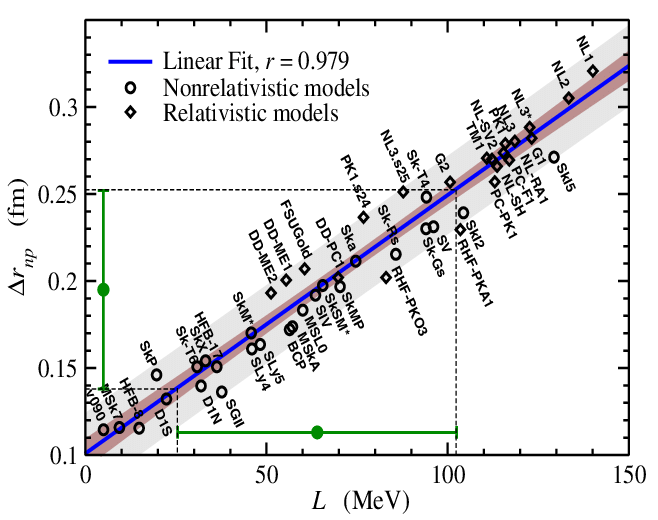
\includegraphics[width=0.50\textwidth]{Introduzione/color-online-Neutron-skin-of-208-Pb-against-slope-of-the-symmetry-energy-The-linear.png}
 \caption{Neutron skin thickness of $^{208}Pb$ as a function of the slope of the symmetry energy $L$.}
 \end{figure}
 
A strong correlation is present between the values of the symmetry energy and the neutron skin thickness, and measuring the second give the access to the first. 

\section{Parity-violating scattering experiment}

\commento{This section is for describing the way it's possible to extract the neutron skin thickness. Here I have to mention the weak form factor and the important fact that the neutrons are more important than the protons in the parity-violating scattering, because of the weak mixing angle.}

\section{Transverse asymmetry}

\commento{Here we have to introduce the aim of this thesis: the transverse asymmetry is a source of background for the parity-violating experiments. Furthermore the theory is not working well for some nuclei ($^{208}Pb$), so mention PREX paper about the last measurement on carbon and lead, the problem that they measure $0$ transverse asymmetry.}

\subsection{Motivation}
\commento{Here present all the motivation for this thesis, so the fact that we want to measure the rates on lead for the future experiment, test the new electronics, measure another time the trasverse asymmetry on $^{12}C$}

\subsection{Conventions used}
\commento{It could be useful, here, to have a subsection to explain the terminology for this thesis, to avoid misunderstanding.}